\documentclass{assignment}
\usepackage[pdftex]{graphicx}
\usepackage{xcolor}
\definecolor{LightGray}{gray}{0.95}
\usepackage{fancyvrb}
\usepackage{float}
\usepackage[letterpaper, margin = 2.5cm]{geometry}
\usepackage[T1]{fontenc}
\usepackage{amsmath, amsfonts, amssymb}
\usepackage{hyperref, url}
\usepackage{fancyhdr}

\newcommand{\n}{\vspace{0.2cm}}
\def\u{\mathbf u}
\def\v{\mathbf v}
\def\w{\mathbf w}
\def\x{\mathbf x}
\def\y{\mathbf y}
\def\z{\mathbf z}

\student{Fletcher Gornick}
\semester{Spring 2024}
\date{\today}

\courselabel{CSCI 5607}
\exercisesheet{Assignment 1A}{Ray Casting}

\school{College of Science and Engineering}
\university{University of Minnesota, Twin Cities}

\begin{document}

\begin{enumerate}
 \item How does the apparent rotation of the scene with respect to the viewpoint change with changes in the direction of the `up’ vector? \n\\
       take view-vector \(\x\) and up-vector \(\y\), and let the view orientation be defined by unit vectors \(\u\), \(\v\), \(\w\):
       \[\w = \frac{-\x}{\lVert \x \rVert}, \quad \u = \frac{\y \times \w}{\lVert \y \times \w \rVert}, \quad \v = \w \times \u.\]
       We can think of vector \(\u\) as our ``right'' direction vector, this is directly dependent on our up-vector \(\y\).  Now let's take the orthogonal decomposition of \(\y\) with respect to \(\w\), \(\y = \alpha \w + \beta \z\).  We can use this decomposition to relate \(\u\) to \(\w\) and \(\z\):
       \[\u \propto  \y \times \w = (\alpha \w + \beta \z) \times \w = \alpha (\w \times \w) + \beta (\z \times \w) = \beta (\z \times \w), \; \z \perp \w.\]
       As you can see, this cross product is strictly dependent on the part of \(\y\) that's orthogonal to \(\w\), meaning any change in \(\y\) along our viewing direction results in no rotation of our scecne (although if \(\y\) is parallel to \(\w\), then \(\u\) is undefined).

       In the figures below, I ran my raytracer with identical input files, the only thing I changed was the up-vector \(\y\).  Here are the results (viewdir = \((0,0,-1)\) by the way):

       \begin{figure}[H]
        \centering
        \begin{minipage}[c]{0.3\linewidth}
         \centering
         
\includegraphics[width=4cm]{img/e1a.png}
         \caption{updir = \((0,1,0)\)}
        \end{minipage}
        \begin{minipage}[c]{0.3\linewidth}
         \centering
         
\includegraphics[width=4cm]{img/e1b.png}
         \caption{updir = \((0,1,1)\)}
        \end{minipage}
        \begin{minipage}[c]{0.3\linewidth}
         \centering
         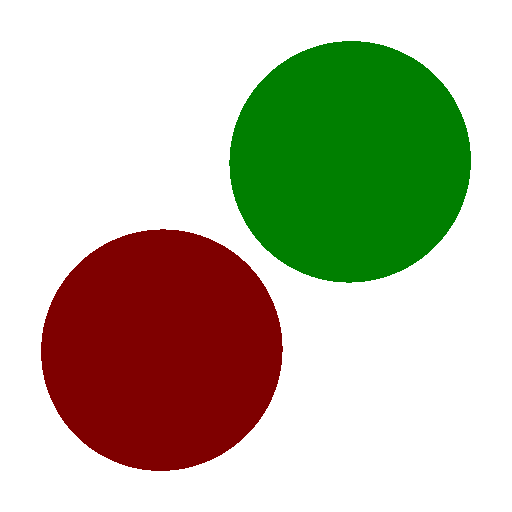
\includegraphics[width=4cm]{img/e1c.png}
         \caption{updir = \((1,1,0)\)}
        \end{minipage}
       \end{figure}

 \item How do changes in field of view settings affect the appearance of the scene in your rendered image? \n\\
       The most notable changes is the size difference of objects at different distances, and the apparent ``zoom'' of the rendered image. \n \\
       With ``zoom'', the wider your field of view, the more surroundings you can see.  So if something is right in front of you, it will appear pretty small because you're seeing your surroundings too, this gives a ``zoomed out'' feel.  With a narrow field of view, you can really only see what's right in front of you, but since that's the case it feels much closer, this is like ``zooming in''. \n\\
       With object overlap, a wide field of view means that objects that are closer will more easily obstruct the veiw of objects further away, this gives the feeling of a fish lens (it essentially is just that).  Whereas if your field of view is more narrow, each individual ray shooting from the origin doesn't differ much from the last, making distance to the camera less meaningful.  You can see an example of this on the next page.

       \begin{figure}[H]
        \centering
        \begin{minipage}[c]{0.3\linewidth}
         \centering
         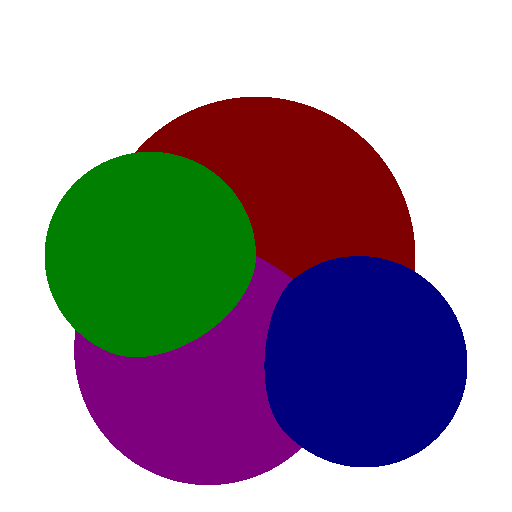
\includegraphics[width=4cm]{img/e2a.png}
         \caption{hfov = \(45^\circ\)}
        \end{minipage}
        \begin{minipage}[c]{0.3\linewidth}
         \centering
         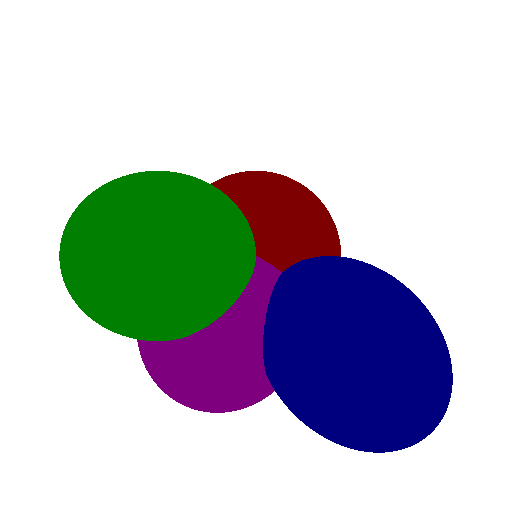
\includegraphics[width=4cm]{img/e2b.png}
         \caption{hfov = \(120^\circ\)}
        \end{minipage}
        \begin{minipage}[c]{0.3\linewidth}
         \centering
         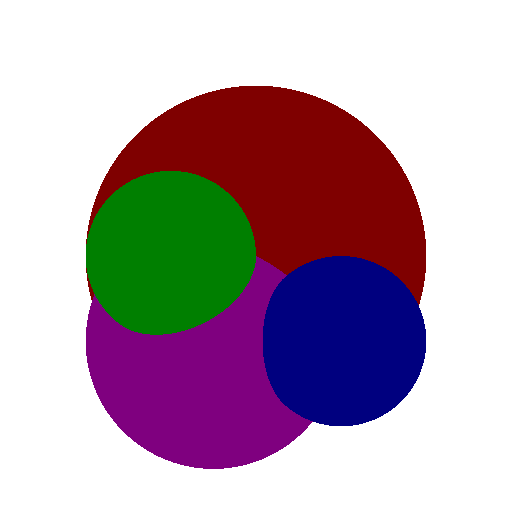
\includegraphics[width=4cm]{img/e2c.png}
         \caption{hfov = \(0^\circ\) (parallel)}
        \end{minipage}
       \end{figure}


 \item How can the viewing parameters (e.g. the camera location, field of view settings, …) be adjusted to achieve a less exaggerated vs more exaggerated amount of apparent perspective distortion in your image? \n\\
       Generally, up close and wider viewing angle leads to more perspective distortion, and far away with narrower viewing angle yields less perspective distortion.

       \begin{figure}[H]
        \centering
        \begin{minipage}[c]{0.3\linewidth}
         \centering
         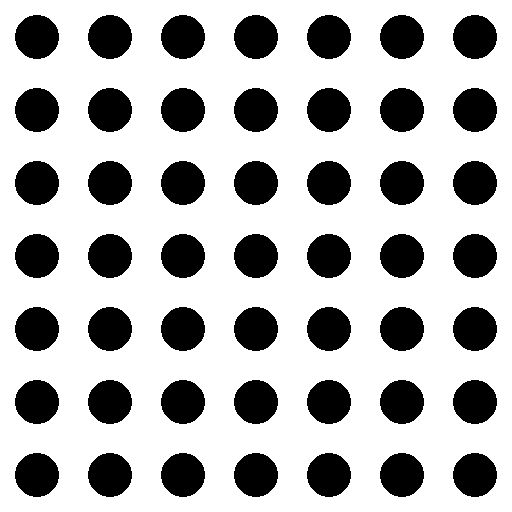
\includegraphics[width=4cm]{img/e3a.png}
         \caption{hfov = \(0^\circ\), \(d = \infty\)}
        \end{minipage}
        \begin{minipage}[c]{0.3\linewidth}
         \centering
         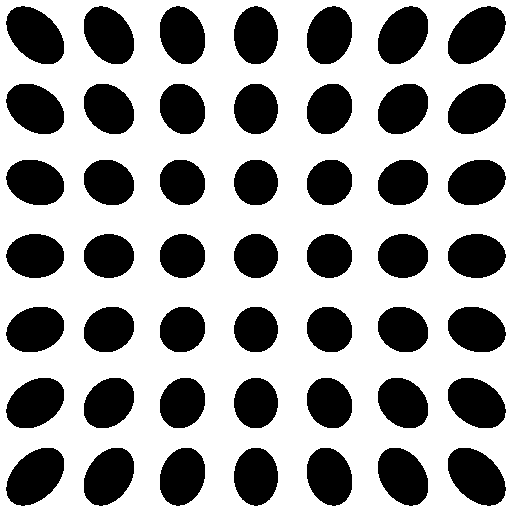
\includegraphics[width=4cm]{img/e3b.png}
         \caption{hfov = \(90^\circ\), \(d = 4\)}
        \end{minipage}
        \begin{minipage}[c]{0.3\linewidth}
         \centering
         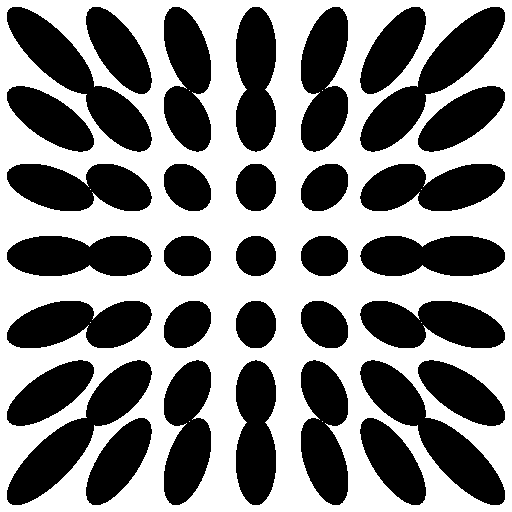
\includegraphics[width=4cm]{img/e3c.png}
         \caption{hfov = \(120^\circ\), \(d = 1.2\)}
        \end{minipage}
       \end{figure}

       Note: all these images were generated from the Assignment 1A raytracer program.
\end{enumerate}
\end{document}
